\documentclass[a4paper,12pt]{article}

\usepackage[utf8x]{inputenc}
\usepackage[T2A]{fontenc}
\usepackage[english, russian]{babel}

% Опционно, требует  apt-get install scalable-cyrfonts.*
% и удаления одной строчки в cyrtimes.sty
% Сточку не удалять!
% \usepackage{cyrtimes}

% Картнки и tikz
\usepackage{graphicx}
\usepackage{tikz}
\usetikzlibrary{snakes,arrows,shapes}


% Некоторая русификация.
\usepackage{misccorr}
\usepackage{indentfirst}
\renewcommand{\labelitemi}{\normalfont\bfseries{--}}

% Увы, поля придётся уменьшить из-за листингов.
\topmargin -1cm
\oddsidemargin -0.5cm
\evensidemargin -0.5cm
\textwidth 17cm
\textheight 24cm

\sloppy

% Оглавление в PDF
\usepackage[
bookmarks=true,
colorlinks=true, linkcolor=black, anchorcolor=black, citecolor=black, menucolor=black,filecolor=black, urlcolor=black,
unicode=true
]{hyperref}

% Для исходного кода в тексте
\newcommand{\Code}[1]{\texttt{#1}}

\usepackage{verbatim}
\usepackage{fancyvrb}
\fvset{frame=leftline, fontsize=\small, framerule=0.4mm, rulecolor=\color{darkgray}, commandchars=\\\{\}}
\renewcommand{\theFancyVerbLine}{\small\arabic{FancyVerbLine}}


\title{Отчёт по лабораторной работе \\ <<IP-маршрутизация>>}
\author{Trung Luong}

\begin{document}

\maketitle

\tableofcontents

% Текст отчёта должен быть читаемым!!! Написанное здесь является рыбой.

\section{Топология сети}

Топология сети и использыемые IP-адреса показаны на рис.~\ref{fig:network}.

\begin{figure}
\centering
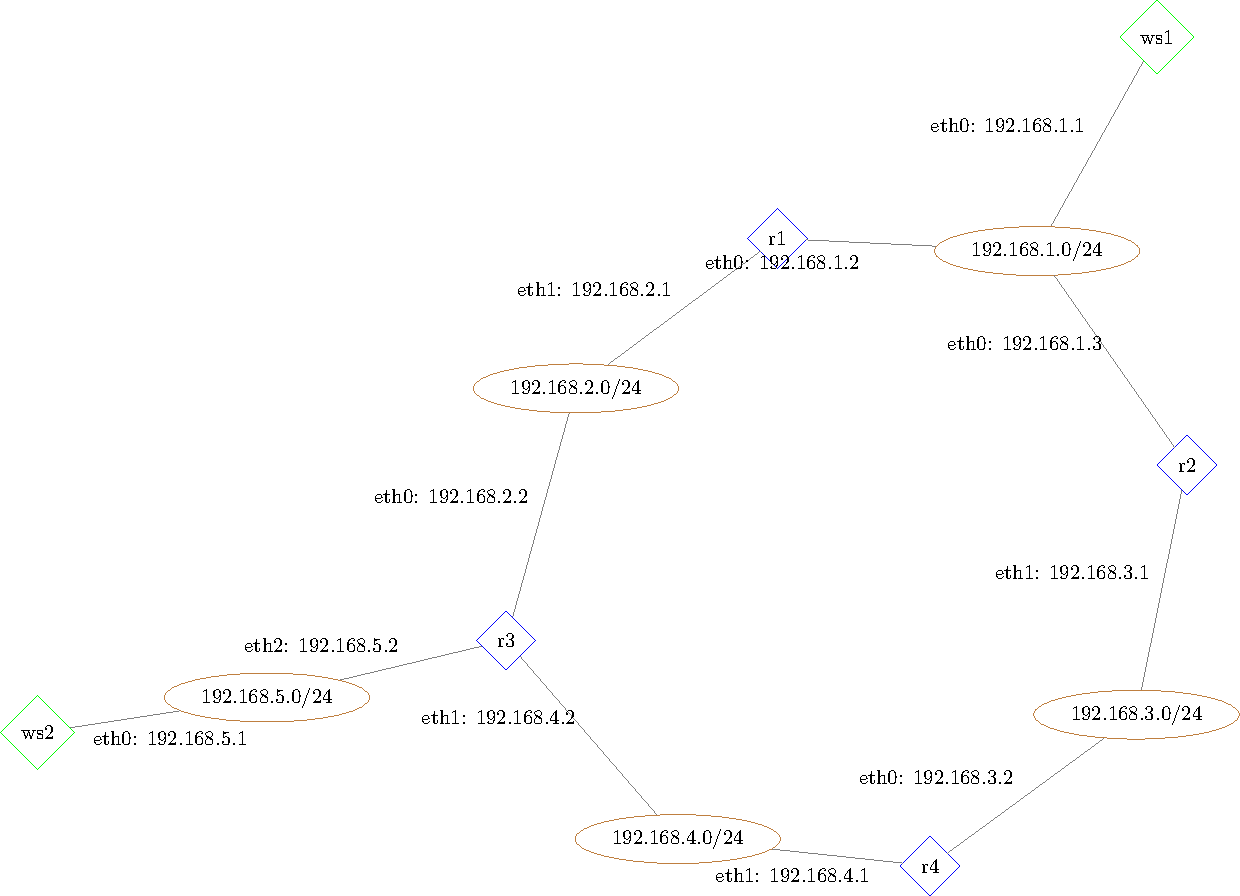
\includegraphics[width=\textwidth]{includes/network_gv.pdf}
\caption{Топология сети}
\label{fig:network}
\end{figure}


\section{Назначение IP-адресов}

Ниже приведён файл настройки протокола IP маршрутизатора (указать, какого).

\begin{Verbatim}
Сюда нужно поместить характерный /etc/network/interfaces маршрутизатора
\end{Verbatim}

Ниже приведён файл настройки протокола IP рабочей станции (указать, какой).

\begin{Verbatim}
Сюда нужно поместить характерный /etc/network/interfaces рабочей станции
\end{Verbatim}


\section{Таблица маршрутизации}

Вывести (командой ip r) таблицу маршрутизации для \textbf{r1}.

\begin{Verbatim}
192.168.5.0/24 via 192.168.2.2 dev eth1 
192.168.4.0/24 via 192.168.2.2 dev eth1 
192.168.3.0/24 via 192.168.2.2 dev eth1 
192.168.2.0/24 dev eth1  proto kernel  scope link  src 192.168.2.1 
192.168.1.0/24 dev eth0  proto kernel  scope link  src 192.168.1.2 
\end{Verbatim}

Вывести (командой ip r) таблицу маршрутизации для \textbf{r2}.

\begin{Verbatim}
192.168.5.0/24 via 192.168.3.2 dev eth1 
192.168.4.0/24 via 192.168.3.2 dev eth1 
192.168.3.0/24 dev eth1  proto kernel  scope link  src 192.168.3.1 
192.168.2.0/24 via 192.168.3.2 dev eth1 
192.168.1.0/24 dev eth0  proto kernel  scope link  src 192.168.1.3
\end{Verbatim}

Вывести (командой ip r) таблицу маршрутизации для \textbf{r3}.

\begin{Verbatim}
192.168.5.0/24 dev eth2  proto kernel  scope link  src 192.168.5.2 
192.168.4.0/24 dev eth1  proto kernel  scope link  src 192.168.4.2 
192.168.3.0/24 via 192.168.4.1 dev eth1 
192.168.2.0/24 dev eth0  proto kernel  scope link  src 192.168.2.2 
192.168.1.0/24 via 192.168.2.1 dev eth0 
\end{Verbatim}

Вывести (командой ip r) таблицу маршрутизации для \textbf{r4}.

\begin{Verbatim}
192.168.5.0/24 via 192.168.4.2 dev eth1 
192.168.4.0/24 dev eth1  proto kernel  scope link  src 192.168.4.1 
192.168.3.0/24 dev eth0  proto kernel  scope link  src 192.168.3.2 
192.168.2.0/24 via 192.168.4.2 dev eth1 
192.168.1.0/24 via 192.168.4.2 dev eth1 
\end{Verbatim}

Вывести (командой ip r) таблицу маршрутизации для \textbf{ws1}.

\begin{Verbatim}
192.168.1.0/24 dev eth0  proto kernel  scope link  src 192.168.1.1 
default via 192.168.1.2 dev eth0 
\end{Verbatim}

Вывести (командой ip r) таблицу маршрутизации для \textbf{ws2}.

\begin{Verbatim}
192.168.5.0/24 dev eth0  proto kernel  scope link  src 192.168.5.1 
default via 192.168.5.2 dev eth0
\end{Verbatim}


\section{Проверка настройки сети}

Вывод \textbf{traceroute} от узла \textbf{ws1} такого-то до такого-то при нормальной работе сети.

\begin{Verbatim}
ws1:~# traceroute -n 192.168.5.1
traceroute to 192.168.5.1 (192.168.5.1), 64 hops max, 40 byte packets
 1  192.168.1.2  1 ms  1 ms  1 ms
 2  192.168.2.2  12 ms  1 ms  1 ms
 3  192.168.5.1  12 ms  1 ms  1 ms
\end{Verbatim}

Вывод \textbf{traceroute} от узла \textbf{ws2} такого-то до такого-то при нормальной работе сети.

\begin{Verbatim}
ws2:~# traceroute -n 192.168.1.1
traceroute to 192.168.1.1 (192.168.1.1), 64 hops max, 40 byte packets
 1  192.168.5.2  1 ms  0 ms  1 ms
 2  192.168.2.1  1 ms  1 ms  1 ms
 3  192.168.1.1  1 ms  1 ms  1 ms
\end{Verbatim}


\section{Маршрутизация}

% На пути здесь достаточно быть одному аршрутизатору!

Тестирование на MAC-адреса интерфейс \textbf{r1}:

\begin{Verbatim}
192.168.5.0/24 via 192.168.2.2 dev eth1 
192.168.4.0/24 via 192.168.2.2 dev eth1 
192.168.3.0/24 via 192.168.2.2 dev eth1 
192.168.2.0/24 dev eth1  proto kernel  scope link  src 192.168.2.1 
192.168.1.0/24 dev eth0  proto kernel  scope link  src 192.168.1.2 
\end{Verbatim}

Тестирование на MAC-адреса интерфейс \textbf{r3}:

\begin{Verbatim}
192.168.5.0/24 dev eth2  proto kernel  scope link  src 192.168.5.2 
192.168.4.0/24 dev eth1  proto kernel  scope link  src 192.168.4.2 
192.168.3.0/24 via 192.168.4.1 dev eth1 
192.168.2.0/24 dev eth0  proto kernel  scope link  src 192.168.2.2 
192.168.1.0/24 via 192.168.2.1 dev eth0 
\end{Verbatim}

Для стирания кеша ARP, выполняется следующая команда: 
\begin{Verbatim}
ip n flush all
\end{Verbatim}

Далее показана отправка пакета на маршрутизатор (косвенная маршрутизация). 

\begin{Verbatim}
a6:f9:52:b6:1e:69 > ff:ff:ff:ff:ff:ff, ethertype ARP (0x0806), length 42: arp who-has 192.168.1.2 tell 192.168.1.1
0e:ab:f8:0c:10:4b > a6:f9:52:b6:1e:69, ethertype ARP (0x0806), length 42: arp reply 192.168.1.2 is-at 0e:ab:f8:0c:10:4b
a6:f9:52:b6:1e:69 > 0e:ab:f8:0c:10:4b, ethertype IPv4 (0x0800), length 98: 192.168.1.1 > 192.168.5.1: ICMP echo request, id 11778, seq 1, length 64
0e:ab:f8:0c:10:4b > a6:f9:52:b6:1e:69, ethertype IPv4 (0x0800), length 98: 192.168.5.1 > 192.168.1.1: ICMP echo reply, id 11778, seq 1, length 64
0e:ab:f8:0c:10:4b > a6:f9:52:b6:1e:69, ethertype ARP (0x0806), length 42: arp who-has 192.168.1.1 tell 192.168.1.2
a6:f9:52:b6:1e:69 > 0e:ab:f8:0c:10:4b, ethertype ARP (0x0806), length 42: arp reply 192.168.1.1 is-at a6:f9:52:b6:1e:69
\end{Verbatim}

\begin{Verbatim}
fa:de:dc:30:96:57 > ff:ff:ff:ff:ff:ff, ethertype ARP (0x0806), length 42: arp who-has 192.168.2.2 tell 192.168.2.1
ee:97:f2:ab:47:0c > fa:de:dc:30:96:57, ethertype ARP (0x0806), length 42: arp reply 192.168.2.2 is-at ee:97:f2:ab:47:0c
fa:de:dc:30:96:57 > ee:97:f2:ab:47:0c, ethertype IPv4 (0x0800), length 98: 192.168.1.1 > 192.168.5.1: ICMP echo request, id 11778, seq 1, length 64
ee:97:f2:ab:47:0c > fa:de:dc:30:96:57, ethertype IPv4 (0x0800), length 98: 192.168.5.1 > 192.168.1.1: ICMP echo reply, id 11778, seq 1, length 64
ee:97:f2:ab:47:0c > fa:de:dc:30:96:57, ethertype ARP (0x0806), length 42: arp who-has 192.168.2.1 tell 192.168.2.2
fa:de:dc:30:96:57 > ee:97:f2:ab:47:0c, ethertype ARP (0x0806), length 42: arp reply 192.168.2.1 is-at fa:de:dc:30:96:57
\end{Verbatim}

Затем маршрутизатор отправил его далее.

\begin{Verbatim}
c2:57:e2:f3:3f:00 > ff:ff:ff:ff:ff:ff, ethertype ARP (0x0806), length 42: arp who-has 192.168.5.1 tell 192.168.5.2
da:53:12:09:ea:4e > c2:57:e2:f3:3f:00, ethertype ARP (0x0806), length 42: arp reply 192.168.5.1 is-at da:53:12:09:ea:4e
c2:57:e2:f3:3f:00 > da:53:12:09:ea:4e, ethertype IPv4 (0x0800), length 98: 192.168.1.1 > 192.168.5.1: ICMP echo request, id 11778, seq 1, length 64
da:53:12:09:ea:4e > c2:57:e2:f3:3f:00, ethertype IPv4 (0x0800), length 98: 192.168.5.1 > 192.168.1.1: ICMP echo reply, id 11778, seq 1, length 64
da:53:12:09:ea:4e > c2:57:e2:f3:3f:00, ethertype ARP (0x0806), length 42: arp who-has 192.168.5.2 tell 192.168.5.1
c2:57:e2:f3:3f:00 > da:53:12:09:ea:4e, ethertype ARP (0x0806), length 42: arp reply 192.168.5.2 is-at c2:57:e2:f3:3f:00
\end{Verbatim}


\section{Продолжительность жизни пакета}

Сначала написать как и на чём ломали. 

\begin{Verbatim}
r3:~# ip link set eth2 down
r3:~# ip route add 192.168.5.0/24 via 192.168.2.1 dev eth0
\end{Verbatim}

Потом какая-то таблица вышла.

\begin{Verbatim}
192.168.5.0/24 via 192.168.2.1 dev eth0 
192.168.4.0/24 dev eth1  proto kernel  scope link  src 192.168.4.2 
192.168.3.0/24 via 192.168.4.1 dev eth1 
192.168.2.0/24 dev eth0  proto kernel  scope link  src 192.168.2.2 
192.168.1.0/24 via 192.168.2.1 dev eth0 
\end{Verbatim}

Потом что слали.

\begin{Verbatim}
ws1:~# ping 192.168.5.1 -c 1
PING 192.168.5.1 (192.168.5.1) 56(84) bytes of data.
From 192.168.2.2 icmp_seq=1 Time to live exceeded

--- 192.168.5.1 ping statistics ---
1 packets transmitted, 0 received, +1 errors, 100% packet loss, time 0ms
\end{Verbatim}

И что в итоге получилось.

\begin{Verbatim}
r3:~# tcpdump -tnve -i eth0
tcpdump: listening on eth0, link-type EN10MB (Ethernet), capture size 96 bytes
fa:de:dc:30:96:57 > ff:ff:ff:ff:ff:ff, ethertype ARP (0x0806), length 42: arp who-has 192.168.2.2 tell 192.168.2.1
ee:97:f2:ab:47:0c > fa:de:dc:30:96:57, ethertype ARP (0x0806), length 42: arp reply 192.168.2.2 is-at ee:97:f2:ab:47:0c
fa:de:dc:30:96:57 > ee:97:f2:ab:47:0c, ethertype IPv4 (0x0800), length 98: (tos 0x0, ttl 63, id 0, offset 0, flags [DF], proto ICMP (1), length 84) 192.168.1.1 > 192.168.5.1: ICMP echo request, id 11010, seq 1, length 64
ee:97:f2:ab:47:0c > fa:de:dc:30:96:57, ethertype IPv4 (0x0800), length 98: (tos 0x0, ttl 62, id 0, offset 0, flags [DF], proto ICMP (1), length 84) 192.168.1.1 > 192.168.5.1: ICMP echo request, id 11010, seq 1, length 64
fa:de:dc:30:96:57 > ee:97:f2:ab:47:0c, ethertype IPv4 (0x0800), length 98: (tos 0x0, ttl 61, id 0, offset 0, flags [DF], proto ICMP (1), length 84) 192.168.1.1 > 192.168.5.1: ICMP echo request, id 11010, seq 1, length 64
ee:97:f2:ab:47:0c > fa:de:dc:30:96:57, ethertype IPv4 (0x0800), length 98: (tos 0x0, ttl 60, id 0, offset 0, flags [DF], proto ICMP (1), length 84) 192.168.1.1 > 192.168.5.1: ICMP echo request, id 11010, seq 1, length 64
fa:de:dc:30:96:57 > ee:97:f2:ab:47:0c, ethertype IPv4 (0x0800), length 98: (tos 0x0, ttl 59, id 0, offset 0, flags [DF], proto ICMP (1), length 84) 192.168.1.1 > 192.168.5.1: ICMP echo request, id 11010, seq 1, length 64
ee:97:f2:ab:47:0c > fa:de:dc:30:96:57, ethertype IPv4 (0x0800), length 98: (tos 0x0, ttl 58, id 0, offset 0, flags [DF], proto ICMP (1), length 84) 192.168.1.1 > 192.168.5.1: ICMP echo request, id 11010, seq 1, length 64
fa:de:dc:30:96:57 > ee:97:f2:ab:47:0c, ethertype IPv4 (0x0800), length 98: (tos 0x0, ttl 57, id 0, offset 0, flags [DF], proto ICMP (1), length 84) 192.168.1.1 > 192.168.5.1: ICMP echo request, id 11010, seq 1, length 64
ee:97:f2:ab:47:0c > fa:de:dc:30:96:57, ethertype IPv4 (0x0800), length 98: (tos 0x0, ttl 56, id 0, offset 0, flags [DF], proto ICMP (1), length 84) 192.168.1.1 > 192.168.5.1: ICMP echo request, id 11010, seq 1, length 64
fa:de:dc:30:96:57 > ee:97:f2:ab:47:0c, ethertype IPv4 (0x0800), length 98: (tos 0x0, ttl 55, id 0, offset 0, flags [DF], proto ICMP (1), length 84) 192.168.1.1 > 192.168.5.1: ICMP echo request, id 11010, seq 1, length 64
ee:97:f2:ab:47:0c > fa:de:dc:30:96:57, ethertype IPv4 (0x0800), length 98: (tos 0x0, ttl 54, id 0, offset 0, flags [DF], proto ICMP (1), length 84) 192.168.1.1 > 192.168.5.1: ICMP echo request, id 11010, seq 1, length 64
fa:de:dc:30:96:57 > ee:97:f2:ab:47:0c, ethertype IPv4 (0x0800), length 98: (tos 0x0, ttl 53, id 0, offset 0, flags [DF], proto ICMP (1), length 84) 192.168.1.1 > 192.168.5.1: ICMP echo request, id 11010, seq 1, length 64
ee:97:f2:ab:47:0c > fa:de:dc:30:96:57, ethertype IPv4 (0x0800), length 98: (tos 0x0, ttl 52, id 0, offset 0, flags [DF], proto ICMP (1), length 84) 192.168.1.1 > 192.168.5.1: ICMP echo request, id 11010, seq 1, length 64
fa:de:dc:30:96:57 > ee:97:f2:ab:47:0c, ethertype IPv4 (0x0800), length 98: (tos 0x0, ttl 51, id 0, offset 0, flags [DF], proto ICMP (1), length 84) 192.168.1.1 > 192.168.5.1: ICMP echo request, id 11010, seq 1, length 64
ee:97:f2:ab:47:0c > fa:de:dc:30:96:57, ethertype IPv4 (0x0800), length 98: (tos 0x0, ttl 50, id 0, offset 0, flags [DF], proto ICMP (1), length 84) 192.168.1.1 > 192.168.5.1: ICMP echo request, id 11010, seq 1, length 64
fa:de:dc:30:96:57 > ee:97:f2:ab:47:0c, ethertype IPv4 (0x0800), length 98: (tos 0x0, ttl 49, id 0, offset 0, flags [DF], proto ICMP (1), length 84) 192.168.1.1 > 192.168.5.1: ICMP echo request, id 11010, seq 1, length 64
ee:97:f2:ab:47:0c > fa:de:dc:30:96:57, ethertype IPv4 (0x0800), length 98: (tos 0x0, ttl 48, id 0, offset 0, flags [DF], proto ICMP (1), length 84) 192.168.1.1 > 192.168.5.1: ICMP echo request, id 11010, seq 1, length 64
fa:de:dc:30:96:57 > ee:97:f2:ab:47:0c, ethertype IPv4 (0x0800), length 98: (tos 0x0, ttl 47, id 0, offset 0, flags [DF], proto ICMP (1), length 84) 192.168.1.1 > 192.168.5.1: ICMP echo request, id 11010, seq 1, length 64
ee:97:f2:ab:47:0c > fa:de:dc:30:96:57, ethertype IPv4 (0x0800), length 98: (tos 0x0, ttl 46, id 0, offset 0, flags [DF], proto ICMP (1), length 84) 192.168.1.1 > 192.168.5.1: ICMP echo request, id 11010, seq 1, length 64
fa:de:dc:30:96:57 > ee:97:f2:ab:47:0c, ethertype IPv4 (0x0800), length 98: (tos 0x0, ttl 45, id 0, offset 0, flags [DF], proto ICMP (1), length 84) 192.168.1.1 > 192.168.5.1: ICMP echo request, id 11010, seq 1, length 64
ee:97:f2:ab:47:0c > fa:de:dc:30:96:57, ethertype IPv4 (0x0800), length 98: (tos 0x0, ttl 44, id 0, offset 0, flags [DF], proto ICMP (1), length 84) 192.168.1.1 > 192.168.5.1: ICMP echo request, id 11010, seq 1, length 64
fa:de:dc:30:96:57 > ee:97:f2:ab:47:0c, ethertype IPv4 (0x0800), length 98: (tos 0x0, ttl 43, id 0, offset 0, flags [DF], proto ICMP (1), length 84) 192.168.1.1 > 192.168.5.1: ICMP echo request, id 11010, seq 1, length 64
ee:97:f2:ab:47:0c > fa:de:dc:30:96:57, ethertype IPv4 (0x0800), length 98: (tos 0x0, ttl 42, id 0, offset 0, flags [DF], proto ICMP (1), length 84) 192.168.1.1 > 192.168.5.1: ICMP echo request, id 11010, seq 1, length 64
fa:de:dc:30:96:57 > ee:97:f2:ab:47:0c, ethertype IPv4 (0x0800), length 98: (tos 0x0, ttl 41, id 0, offset 0, flags [DF], proto ICMP (1), length 84) 192.168.1.1 > 192.168.5.1: ICMP echo request, id 11010, seq 1, length 64
ee:97:f2:ab:47:0c > fa:de:dc:30:96:57, ethertype IPv4 (0x0800), length 98: (tos 0x0, ttl 40, id 0, offset 0, flags [DF], proto ICMP (1), length 84) 192.168.1.1 > 192.168.5.1: ICMP echo request, id 11010, seq 1, length 64
fa:de:dc:30:96:57 > ee:97:f2:ab:47:0c, ethertype IPv4 (0x0800), length 98: (tos 0x0, ttl 39, id 0, offset 0, flags [DF], proto ICMP (1), length 84) 192.168.1.1 > 192.168.5.1: ICMP echo request, id 11010, seq 1, length 64
ee:97:f2:ab:47:0c > fa:de:dc:30:96:57, ethertype IPv4 (0x0800), length 98: (tos 0x0, ttl 38, id 0, offset 0, flags [DF], proto ICMP (1), length 84) 192.168.1.1 > 192.168.5.1: ICMP echo request, id 11010, seq 1, length 64
fa:de:dc:30:96:57 > ee:97:f2:ab:47:0c, ethertype IPv4 (0x0800), length 98: (tos 0x0, ttl 37, id 0, offset 0, flags [DF], proto ICMP (1), length 84) 192.168.1.1 > 192.168.5.1: ICMP echo request, id 11010, seq 1, length 64
ee:97:f2:ab:47:0c > fa:de:dc:30:96:57, ethertype IPv4 (0x0800), length 98: (tos 0x0, ttl 36, id 0, offset 0, flags [DF], proto ICMP (1), length 84) 192.168.1.1 > 192.168.5.1: ICMP echo request, id 11010, seq 1, length 64
fa:de:dc:30:96:57 > ee:97:f2:ab:47:0c, ethertype IPv4 (0x0800), length 98: (tos 0x0, ttl 35, id 0, offset 0, flags [DF], proto ICMP (1), length 84) 192.168.1.1 > 192.168.5.1: ICMP echo request, id 11010, seq 1, length 64
ee:97:f2:ab:47:0c > fa:de:dc:30:96:57, ethertype IPv4 (0x0800), length 98: (tos 0x0, ttl 34, id 0, offset 0, flags [DF], proto ICMP (1), length 84) 192.168.1.1 > 192.168.5.1: ICMP echo request, id 11010, seq 1, length 64
fa:de:dc:30:96:57 > ee:97:f2:ab:47:0c, ethertype IPv4 (0x0800), length 98: (tos 0x0, ttl 33, id 0, offset 0, flags [DF], proto ICMP (1), length 84) 192.168.1.1 > 192.168.5.1: ICMP echo request, id 11010, seq 1, length 64
ee:97:f2:ab:47:0c > fa:de:dc:30:96:57, ethertype IPv4 (0x0800), length 98: (tos 0x0, ttl 32, id 0, offset 0, flags [DF], proto ICMP (1), length 84) 192.168.1.1 > 192.168.5.1: ICMP echo request, id 11010, seq 1, length 64
fa:de:dc:30:96:57 > ee:97:f2:ab:47:0c, ethertype IPv4 (0x0800), length 98: (tos 0x0, ttl 31, id 0, offset 0, flags [DF], proto ICMP (1), length 84) 192.168.1.1 > 192.168.5.1: ICMP echo request, id 11010, seq 1, length 64
ee:97:f2:ab:47:0c > fa:de:dc:30:96:57, ethertype IPv4 (0x0800), length 98: (tos 0x0, ttl 30, id 0, offset 0, flags [DF], proto ICMP (1), length 84) 192.168.1.1 > 192.168.5.1: ICMP echo request, id 11010, seq 1, length 64
fa:de:dc:30:96:57 > ee:97:f2:ab:47:0c, ethertype IPv4 (0x0800), length 98: (tos 0x0, ttl 29, id 0, offset 0, flags [DF], proto ICMP (1), length 84) 192.168.1.1 > 192.168.5.1: ICMP echo request, id 11010, seq 1, length 64
ee:97:f2:ab:47:0c > fa:de:dc:30:96:57, ethertype IPv4 (0x0800), length 98: (tos 0x0, ttl 28, id 0, offset 0, flags [DF], proto ICMP (1), length 84) 192.168.1.1 > 192.168.5.1: ICMP echo request, id 11010, seq 1, length 64
fa:de:dc:30:96:57 > ee:97:f2:ab:47:0c, ethertype IPv4 (0x0800), length 98: (tos 0x0, ttl 27, id 0, offset 0, flags [DF], proto ICMP (1), length 84) 192.168.1.1 > 192.168.5.1: ICMP echo request, id 11010, seq 1, length 64
ee:97:f2:ab:47:0c > fa:de:dc:30:96:57, ethertype IPv4 (0x0800), length 98: (tos 0x0, ttl 26, id 0, offset 0, flags [DF], proto ICMP (1), length 84) 192.168.1.1 > 192.168.5.1: ICMP echo request, id 11010, seq 1, length 64
fa:de:dc:30:96:57 > ee:97:f2:ab:47:0c, ethertype IPv4 (0x0800), length 98: (tos 0x0, ttl 25, id 0, offset 0, flags [DF], proto ICMP (1), length 84) 192.168.1.1 > 192.168.5.1: ICMP echo request, id 11010, seq 1, length 64
ee:97:f2:ab:47:0c > fa:de:dc:30:96:57, ethertype IPv4 (0x0800), length 98: (tos 0x0, ttl 24, id 0, offset 0, flags [DF], proto ICMP (1), length 84) 192.168.1.1 > 192.168.5.1: ICMP echo request, id 11010, seq 1, length 64
fa:de:dc:30:96:57 > ee:97:f2:ab:47:0c, ethertype IPv4 (0x0800), length 98: (tos 0x0, ttl 23, id 0, offset 0, flags [DF], proto ICMP (1), length 84) 192.168.1.1 > 192.168.5.1: ICMP echo request, id 11010, seq 1, length 64
ee:97:f2:ab:47:0c > fa:de:dc:30:96:57, ethertype IPv4 (0x0800), length 98: (tos 0x0, ttl 22, id 0, offset 0, flags [DF], proto ICMP (1), length 84) 192.168.1.1 > 192.168.5.1: ICMP echo request, id 11010, seq 1, length 64
fa:de:dc:30:96:57 > ee:97:f2:ab:47:0c, ethertype IPv4 (0x0800), length 98: (tos 0x0, ttl 21, id 0, offset 0, flags [DF], proto ICMP (1), length 84) 192.168.1.1 > 192.168.5.1: ICMP echo request, id 11010, seq 1, length 64
ee:97:f2:ab:47:0c > fa:de:dc:30:96:57, ethertype IPv4 (0x0800), length 98: (tos 0x0, ttl 20, id 0, offset 0, flags [DF], proto ICMP (1), length 84) 192.168.1.1 > 192.168.5.1: ICMP echo request, id 11010, seq 1, length 64
fa:de:dc:30:96:57 > ee:97:f2:ab:47:0c, ethertype IPv4 (0x0800), length 98: (tos 0x0, ttl 19, id 0, offset 0, flags [DF], proto ICMP (1), length 84) 192.168.1.1 > 192.168.5.1: ICMP echo request, id 11010, seq 1, length 64
ee:97:f2:ab:47:0c > fa:de:dc:30:96:57, ethertype IPv4 (0x0800), length 98: (tos 0x0, ttl 18, id 0, offset 0, flags [DF], proto ICMP (1), length 84) 192.168.1.1 > 192.168.5.1: ICMP echo request, id 11010, seq 1, length 64
fa:de:dc:30:96:57 > ee:97:f2:ab:47:0c, ethertype IPv4 (0x0800), length 98: (tos 0x0, ttl 17, id 0, offset 0, flags [DF], proto ICMP (1), length 84) 192.168.1.1 > 192.168.5.1: ICMP echo request, id 11010, seq 1, length 64
ee:97:f2:ab:47:0c > fa:de:dc:30:96:57, ethertype IPv4 (0x0800), length 98: (tos 0x0, ttl 16, id 0, offset 0, flags [DF], proto ICMP (1), length 84) 192.168.1.1 > 192.168.5.1: ICMP echo request, id 11010, seq 1, length 64
fa:de:dc:30:96:57 > ee:97:f2:ab:47:0c, ethertype IPv4 (0x0800), length 98: (tos 0x0, ttl 15, id 0, offset 0, flags [DF], proto ICMP (1), length 84) 192.168.1.1 > 192.168.5.1: ICMP echo request, id 11010, seq 1, length 64
ee:97:f2:ab:47:0c > fa:de:dc:30:96:57, ethertype IPv4 (0x0800), length 98: (tos 0x0, ttl 14, id 0, offset 0, flags [DF], proto ICMP (1), length 84) 192.168.1.1 > 192.168.5.1: ICMP echo request, id 11010, seq 1, length 64
fa:de:dc:30:96:57 > ee:97:f2:ab:47:0c, ethertype IPv4 (0x0800), length 98: (tos 0x0, ttl 13, id 0, offset 0, flags [DF], proto ICMP (1), length 84) 192.168.1.1 > 192.168.5.1: ICMP echo request, id 11010, seq 1, length 64
ee:97:f2:ab:47:0c > fa:de:dc:30:96:57, ethertype IPv4 (0x0800), length 98: (tos 0x0, ttl 12, id 0, offset 0, flags [DF], proto ICMP (1), length 84) 192.168.1.1 > 192.168.5.1: ICMP echo request, id 11010, seq 1, length 64
fa:de:dc:30:96:57 > ee:97:f2:ab:47:0c, ethertype IPv4 (0x0800), length 98: (tos 0x0, ttl 11, id 0, offset 0, flags [DF], proto ICMP (1), length 84) 192.168.1.1 > 192.168.5.1: ICMP echo request, id 11010, seq 1, length 64
ee:97:f2:ab:47:0c > fa:de:dc:30:96:57, ethertype IPv4 (0x0800), length 98: (tos 0x0, ttl 10, id 0, offset 0, flags [DF], proto ICMP (1), length 84) 192.168.1.1 > 192.168.5.1: ICMP echo request, id 11010, seq 1, length 64
fa:de:dc:30:96:57 > ee:97:f2:ab:47:0c, ethertype IPv4 (0x0800), length 98: (tos 0x0, ttl 9, id 0, offset 0, flags [DF], proto ICMP (1), length 84) 192.168.1.1 > 192.168.5.1: ICMP echo request, id 11010, seq 1, length 64
ee:97:f2:ab:47:0c > fa:de:dc:30:96:57, ethertype IPv4 (0x0800), length 98: (tos 0x0, ttl 8, id 0, offset 0, flags [DF], proto ICMP (1), length 84) 192.168.1.1 > 192.168.5.1: ICMP echo request, id 11010, seq 1, length 64
fa:de:dc:30:96:57 > ee:97:f2:ab:47:0c, ethertype IPv4 (0x0800), length 98: (tos 0x0, ttl 7, id 0, offset 0, flags [DF], proto ICMP (1), length 84) 192.168.1.1 > 192.168.5.1: ICMP echo request, id 11010, seq 1, length 64
ee:97:f2:ab:47:0c > fa:de:dc:30:96:57, ethertype IPv4 (0x0800), length 98: (tos 0x0, ttl 6, id 0, offset 0, flags [DF], proto ICMP (1), length 84) 192.168.1.1 > 192.168.5.1: ICMP echo request, id 11010, seq 1, length 64
fa:de:dc:30:96:57 > ee:97:f2:ab:47:0c, ethertype IPv4 (0x0800), length 98: (tos 0x0, ttl 5, id 0, offset 0, flags [DF], proto ICMP (1), length 84) 192.168.1.1 > 192.168.5.1: ICMP echo request, id 11010, seq 1, length 64
ee:97:f2:ab:47:0c > fa:de:dc:30:96:57, ethertype IPv4 (0x0800), length 98: (tos 0x0, ttl 4, id 0, offset 0, flags [DF], proto ICMP (1), length 84) 192.168.1.1 > 192.168.5.1: ICMP echo request, id 11010, seq 1, length 64
fa:de:dc:30:96:57 > ee:97:f2:ab:47:0c, ethertype IPv4 (0x0800), length 98: (tos 0x0, ttl 3, id 0, offset 0, flags [DF], proto ICMP (1), length 84) 192.168.1.1 > 192.168.5.1: ICMP echo request, id 11010, seq 1, length 64
ee:97:f2:ab:47:0c > fa:de:dc:30:96:57, ethertype IPv4 (0x0800), length 98: (tos 0x0, ttl 2, id 0, offset 0, flags [DF], proto ICMP (1), length 84) 192.168.1.1 > 192.168.5.1: ICMP echo request, id 11010, seq 1, length 64
fa:de:dc:30:96:57 > ee:97:f2:ab:47:0c, ethertype IPv4 (0x0800), length 98: (tos 0x0, ttl 1, id 0, offset 0, flags [DF], proto ICMP (1), length 84) 192.168.1.1 > 192.168.5.1: ICMP echo request, id 11010, seq 1, length 64
ee:97:f2:ab:47:0c > fa:de:dc:30:96:57, ethertype IPv4 (0x0800), length 126: (tos 0xc0, ttl 64, id 50257, offset 0, flags [none], proto ICMP (1), length 112) 192.168.2.2 > 192.168.1.1: ICMP time exceeded in-transit, length 92
	(tos 0x0, ttl 1, id 0, offset 0, flags [DF], proto ICMP (1), length 84) 192.168.1.1 > 192.168.5.1: ICMP echo request, id 11010, seq 1, length 64
ee:97:f2:ab:47:0c > fa:de:dc:30:96:57, ethertype ARP (0x0806), length 42: arp who-has 192.168.2.1 tell 192.168.2.2
fa:de:dc:30:96:57 > ee:97:f2:ab:47:0c, ethertype ARP (0x0806), length 42: arp reply 192.168.2.1 is-at fa:de:dc:30:96:57
\end{Verbatim}

И кто в итоге отравил сообщение о завершении жизни.

\begin{Verbatim}
ws1:~# traceroute -n 192.168.5.1
traceroute to 192.168.5.1 (192.168.5.1), 64 hops max, 40 byte packets
 1  192.168.1.2  6 ms  0 ms  0 ms
 2  192.168.2.2  11 ms  0 ms  0 ms
 3  192.168.1.2  0 ms  0 ms  0 ms
 4  192.168.2.2  0 ms  0 ms  0 ms
 5  * 192.168.1.2  1 ms  0 ms
 6  192.168.2.2  0 ms  0 ms  0 ms
 7  192.168.1.2  0 ms *  2 ms
 8  192.168.2.2  2 ms  1 ms  1 ms
 9  192.168.1.2  1 ms  1 ms *
10  192.168.2.2  1 ms  1 ms  0 ms
11  192.168.1.2  1 ms  0 ms  0 ms
12  * 192.168.2.2  2 ms  1 ms
13  192.168.1.2  1 ms  1 ms  1 ms
14  192.168.2.2  1 ms *  1 ms
15  192.168.1.2  1 ms  1 ms  1 ms
16  192.168.2.2  1 ms  1 ms *
17  192.168.1.2  1 ms  1 ms  1 ms
18  192.168.2.2  1 ms  1 ms  1 ms
19  * 192.168.1.2  2 ms  2 ms
20  192.168.2.2  2 ms  2 ms  2 ms
21  192.168.1.2  1 ms *  1 ms
22  192.168.2.2  1 ms  1 ms  1 ms
23  192.168.1.2  1 ms  1 ms *
24  192.168.2.2  1 ms  1 ms  1 ms
25  192.168.1.2  1 ms  1 ms  1 ms
26  * 192.168.2.2  1 ms  1 ms
27  192.168.1.2  1 ms  1 ms  1 ms
28  192.168.2.2  1 ms *  2 ms
29  192.168.1.2  1 ms  1 ms  1 ms
30  192.168.2.2  1 ms  1 ms *
31  192.168.1.2  5 ms  2 ms  1 ms
32  192.168.2.2  1 ms  1 ms  1 ms
33  * 192.168.1.2  2 ms  2 ms
34  192.168.2.2  2 ms  2 ms  2 ms
35  192.168.1.2  2 ms *  2 ms
36  192.168.2.2  1 ms  1 ms  1 ms
37  192.168.1.2  1 ms  1 ms *
38  192.168.2.2  2 ms  1 ms  1 ms
39  192.168.1.2  1 ms  2 ms  1 ms
40  * 192.168.2.2  2 ms  1 ms
41  192.168.1.2  1 ms  1 ms  1 ms
42  192.168.2.2  2 ms *  2 ms
43  192.168.1.2  1 ms  2 ms  1 ms
44  192.168.2.2  1 ms  1 ms *
45  192.168.1.2  2 ms  2 ms  2 ms
46  192.168.2.2  2 ms  2 ms  2 ms
47  * 192.168.1.2  2 ms  2 ms
48  192.168.2.2  2 ms  2 ms  2 ms
49  192.168.1.2  2 ms *  2 ms
50  192.168.2.2  2 ms  2 ms  2 ms
51  192.168.1.2  2 ms  2 ms *
52  192.168.2.2  2 ms  2 ms  2 ms
53  192.168.1.2  2 ms  2 ms  2 ms
54  * 192.168.2.2  4 ms  3 ms
55  192.168.1.2  3 ms  3 ms  3 ms
56  192.168.2.2  3 ms *  8 ms
57  192.168.1.2  4 ms  2 ms  2 ms
58  192.168.2.2  2 ms  2 ms *
59  192.168.1.2  8 ms  7 ms  4 ms
60  192.168.2.2  3 ms  3 ms  2 ms
61  * 192.168.1.2  7 ms  4 ms
62  192.168.2.2  4 ms  3 ms  3 ms
63  192.168.1.2  2 ms *  3 ms
64  192.168.2.2  2 ms  2 ms  2 ms
\end{Verbatim}


\section{Изучение IP-фрагментации}

Написать, на каких узлах и как изменяли MTU.

\begin{Verbatim}
Изменение MTU
\end{Verbatim}

\begin{Verbatim}
Изменение MTU
\end{Verbatim}

% Напоминаем, что PMTU следует отключить!

Какие команды давали для тестирования и где.

\begin{Verbatim}
r1:~# ip link set dev eth1 mtu 600
r3:~# ip link set dev eth0 mtu 600

echo 1 > /proc/sys/net/ipv4/ip_no_pmtu_disc

ws1:~# ping 192.168.5.1 -c 1 -s 1000
\end{Verbatim}

Вывод \textbf{tcpdump} на маршрутизаторе перед сетью с уменьшенным MTU.

% Вывод в ширину можно и сократить, удалив несущественные моменты!

\begin{Verbatim}
r1:~# tcpdump -tnv -i eth0 icmp
tcpdump: listening on eth0, link-type EN10MB (Ethernet), capture size 96 bytes
IP (tos 0x0, ttl 64, id 29245, offset 0, flags [none], proto ICMP (1), length 1028) 192.168.1.1 > 192.168.5.1: ICMP echo request, id 11266, seq 1, length 1008
IP (tos 0x0, ttl 62, id 39740, offset 0, flags [none], proto ICMP (1), length 1028) 192.168.5.1 > 192.168.1.1: ICMP echo reply, id 11266, seq 1, length 1008
\end{Verbatim}

Вывод \textbf{tcpdump} на маршрутизаторе после сети с уменьшенным MTU.

% Вывод в ширину можно и сократить, удалив несущественные моменты!

\begin{Verbatim}
r3:~# tcpdump -tnv -i eth0 icmp
tcpdump: listening on eth0, link-type EN10MB (Ethernet), capture size 96 bytes
IP (tos 0x0, ttl 63, id 29245, offset 0, flags [+], proto ICMP (1), length 596) 192.168.1.1 > 192.168.5.1: ICMP echo request, id 11266, seq 1, length 576
IP (tos 0x0, ttl 63, id 29245, offset 576, flags [none], proto ICMP (1), length 452) 192.168.1.1 > 192.168.5.1: icmp
IP (tos 0x0, ttl 63, id 39740, offset 0, flags [+], proto ICMP (1), length 596) 192.168.5.1 > 192.168.1.1: ICMP echo reply, id 11266, seq 1, length 576
IP (tos 0x0, ttl 63, id 39740, offset 576, flags [none], proto ICMP (1), length 452) 192.168.5.1 > 192.168.1.1: icmp
\end{Verbatim}


Вывод \textbf{tcpdump} на узле получателя.

\begin{Verbatim}
ws2:~# tcpdump -tnv -i eth0 icmp
tcpdump: listening on eth0, link-type EN10MB (Ethernet), capture size 96 bytes
IP (tos 0x0, ttl 62, id 29245, offset 0, flags [none], proto ICMP (1), length 1028) 192.168.1.1 > 192.168.5.1: ICMP echo request, id 11266, seq 1, length 1008
IP (tos 0x0, ttl 64, id 39740, offset 0, flags [none], proto ICMP (1), length 1028) 192.168.5.1 > 192.168.1.1: ICMP echo reply, id 11266, seq 1, length 1008
\end{Verbatim}


\section{Отсутствие сети}

Аналогично опишите опыт, когда маршрутизатор отсылает сообщение об отстутствии с сети.
С командами и выводом, мак адреса не нужны.

\begin{Verbatim}
ws1:~# ping 192.168.6.1 -c 1
PING 192.168.6.1 (192.168.6.1) 56(84) bytes of data.
From 192.168.1.2 icmp_seq=1 Destination Net Unreachable

--- 192.168.6.1 ping statistics ---
1 packets transmitted, 0 received, +1 errors, 100% packet loss, time 0ms

r1:~# tcpdump -n -i eth0 icmp
tcpdump: verbose output suppressed, use -v or -vv for full protocol decode
listening on eth0, link-type EN10MB (Ethernet), capture size 96 bytes
22:07:14.304125 IP 192.168.1.1 > 192.168.6.1: ICMP echo request, id 11010, seq 1, length 64
22:07:14.304143 IP 192.168.1.2 > 192.168.1.1: ICMP net 192.168.6.1 unreachable, length 92
\end{Verbatim}


\section{Отсутствие IP-адреса в сети}

Аналогично опишите опыт, когда маршрутизатор отсылает сообщение об отстутствии требуемого IP-адреса в сети.
С командами и выводом, мак адреса не нужны.

\begin{Verbatim}
ws1:~# ping 192.168.5.4 -c 1
PING 192.168.5.4 (192.168.5.4) 56(84) bytes of data.
From 192.168.2.2 icmp_seq=1 Destination Host Unreachable

--- 192.168.5.4 ping statistics ---
1 packets transmitted, 0 received, +1 errors, 100% packet loss, time 0ms

r3:~# tcpdump -n -i eth2
tcpdump: verbose output suppressed, use -v or -vv for full protocol decode
listening on eth2, link-type EN10MB (Ethernet), capture size 96 bytes
22:11:10.233182 arp who-has 192.168.5.4 tell 192.168.5.2
22:11:11.235214 arp who-has 192.168.5.4 tell 192.168.5.2
22:11:12.235217 arp who-has 192.168.5.4 tell 192.168.5.2
\end{Verbatim}


\end{document}
